%#!/usr/bin/pdflatex \catcode35=14 \input
%\catcode`\#=6

\documentclass{beamer}
%\usetheme{Default}
\usepackage{verbatim,subcaption,listings}
\usepackage[format=plain]{caption}

\iffalse 
Sections
  Chapter 1
    Who we are, what is vicharak
    Moores law + dennard scaling + von neumann bottleneck
    plea (new, creative, from-first-principles architectures, languages and 
      compute infra) should be created
    overview of existing compute
    4 problems in one slide
    Key ideas (reconfigurability + Heterogeneity (complement not replace))
    Two problems (problem 1 and 2)
  Chapter 2
    Problem 1 - Lack of programming model
    how to reconfigure
    flow based computation
    exemplary dsl + accompanying image
  Chapter 3
    Problem 2 - verilog is hard 
      verilog is the reference line (problems above/below)
      problems above involve simulation/hdl abstractions/hls
      problems below involve synthesis, placement, routing (faster, better)
    we want to solve the problems below verilog 
      cad flow (i.e. operation below verilog) 
    optimization oppurtunities
  Chapter 4
    realizing this goal
    gati
    periplex
    demo
  Conclusion
\fi

\iffalse

Abstract

As Moore's Law's imminent slowdown takes effect, there is a need for innovative
architectures designed from the ground up with both hardware and software in
mind. We describe an architecture along with a family of software programs
(compilers and runtimes) that form the basis of this hardware-software system.
Interoperation with existing compute infrastructure is proposed. The
architecture executes expected functionality not with a fixed instruction set
but by reconfiguring flexible reprogrammable hardware dynamically at computation
time. This reconfiguration, driven by a software compiler, specializes the
hardware for every function but generalizes through reconfiguration. In contrast
to traditional CPU-memory back-and-forth dataflow, this architecture exhibits a
unilateral flow of data with zero instruction overhead, alleviating the von
Neumann bottleneck. Opportunities to improve existing compilers (EDA Software) for
reconfigurable chips (FPGAs) are also discussed.
\fi

\lstset{language=C++, basicstyle=\ttfamily,
                keywordstyle=\color{blue}\ttfamily,
                stringstyle=\color{red}\ttfamily,
                commentstyle=\color{green}\ttfamily,
                tabsize=1,breaklines=true,numbers=left,
                morecomment=[l][\color{magenta}]{\#}}


\title{No-ISA is the Best ISA}
\subtitle{}
\author{Shreeyash Pandey, Rishik Ram Jallarapu}
\institute{Vicharak, India @ vicharak.in}
\date{28th September, 2024}

%\usebackgroundtemplate%
%{%
%    
\includegraphics[width=\paperwidth,height=\paperheight]{logo.eps}%
%}

\usepackage[backend=bibtex,style=numeric]{biblatex}
\addbibresource{slides.bib}

\titlegraphic{
  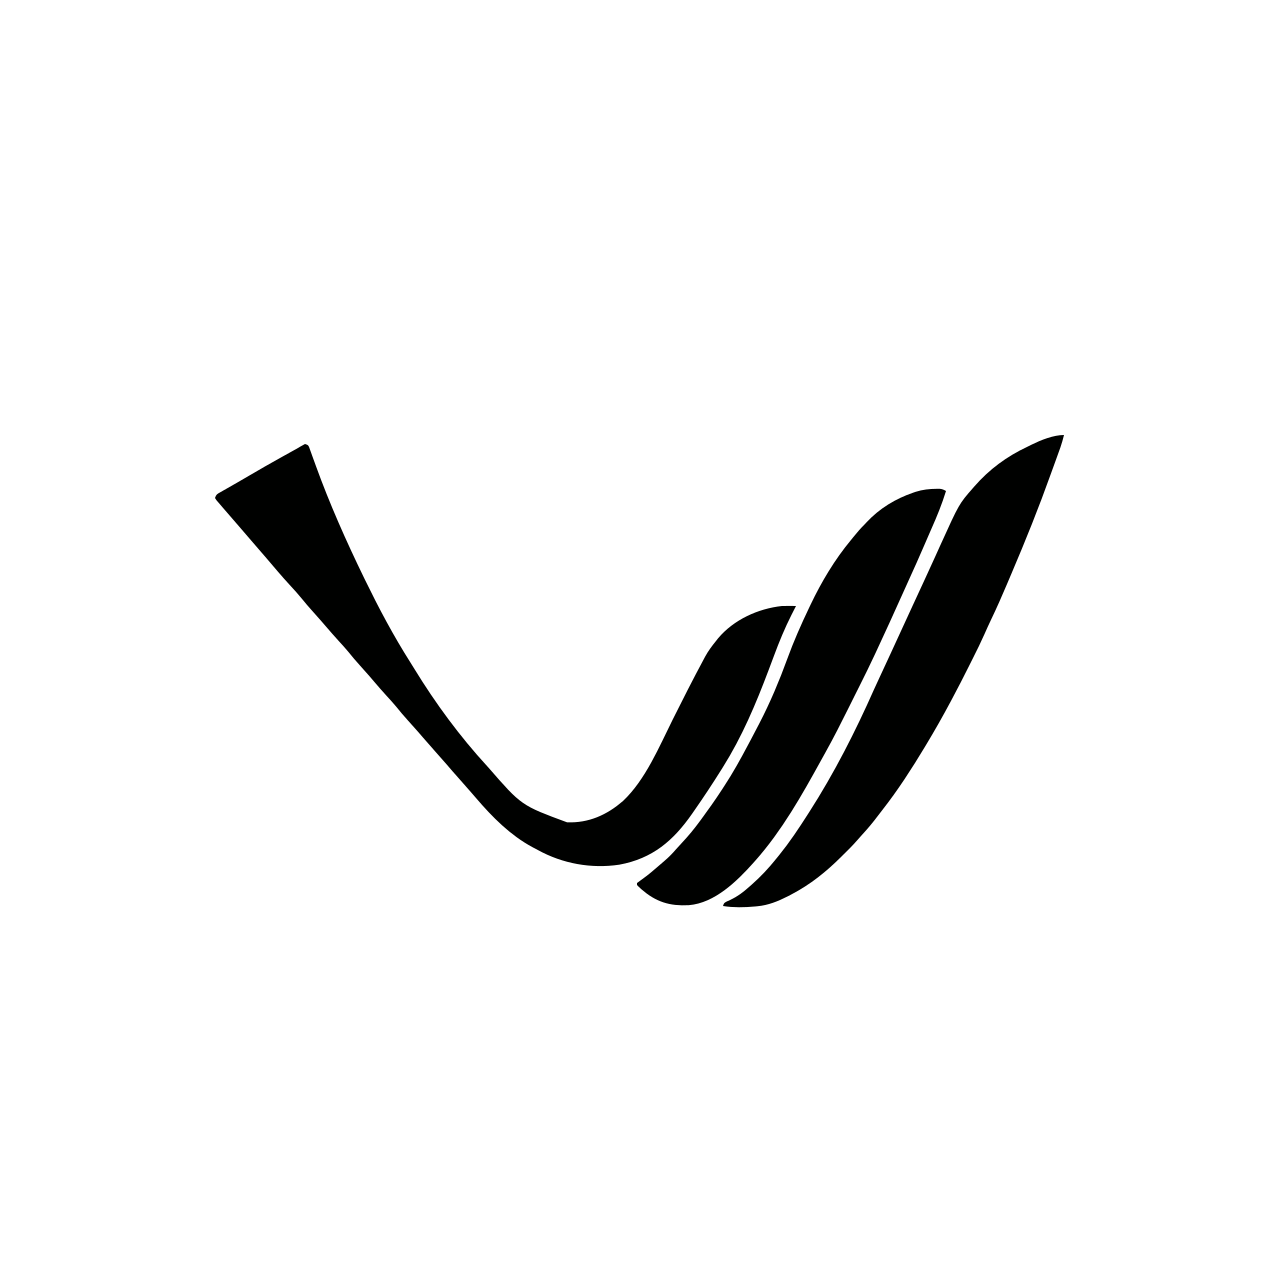
\includegraphics[width=2cm]{images/logo.png}
}


\begin{document}

\begin{frame}
\titlepage
\end{frame}

{
\logo{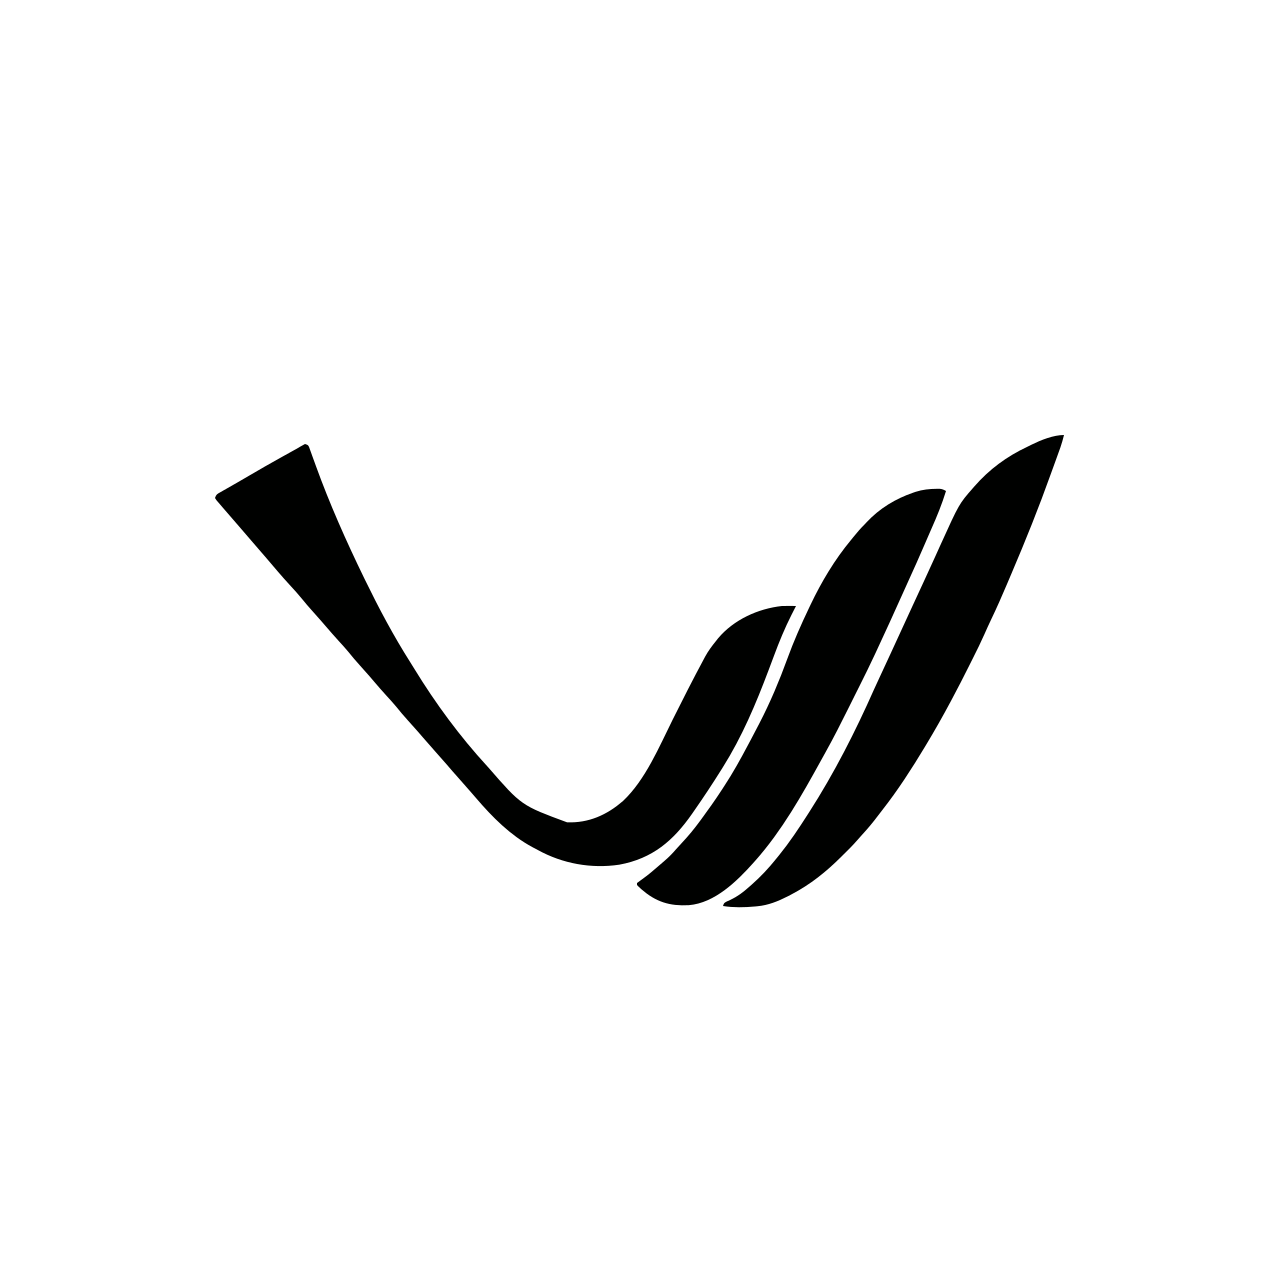
\includegraphics[width=.07\textwidth]{images/logo.png}}

\begin{frame}[fragile]
\frametitle{About us}

  Goals:
  \begin{itemize}
    \item Introduce software-level reconfigurability to hardwares
    \item Consumer and Industrial computing hardware and a new kind of 
      computing ecosystem that can sit on your desk, rest in your palm, or exist in the cloud. 
  \end{itemize}

  For such an ambitious goal, Vicharak is ready to work on every vertical with
  a team of \~{}50 passionate engineers and thinkers deeply entrenched to make this
  vision a reality.

  - Akshar Vastarpara (Founder and CEO, Vicharak)

\framesubtitle{}
\end{frame}

\begin{frame}[fragile]
\frametitle{Contents}

  \begin{itemize}
    \item Chapter 1 - Motivations for our Work
    \item Chapter 2 - Introduction To Reconfigurable And Heterogeneous Computing
    \item Chapter 3 - Need for modern EDA Compilers
    \item Chapter 4 - Work Done Towards Implementation  
  \end{itemize}
\end{frame}

\begin{frame}[c,fragile]
  \frametitle{}
  \centering
  \textbf{Chapter 1}
  \centering
  Motivations for our Work
\end{frame}

\begin{frame}[fragile]
\frametitle{Problems Facing Modern Compute}
  \framesubtitle{Moore's law}

  \begin{figure}
    \centering
    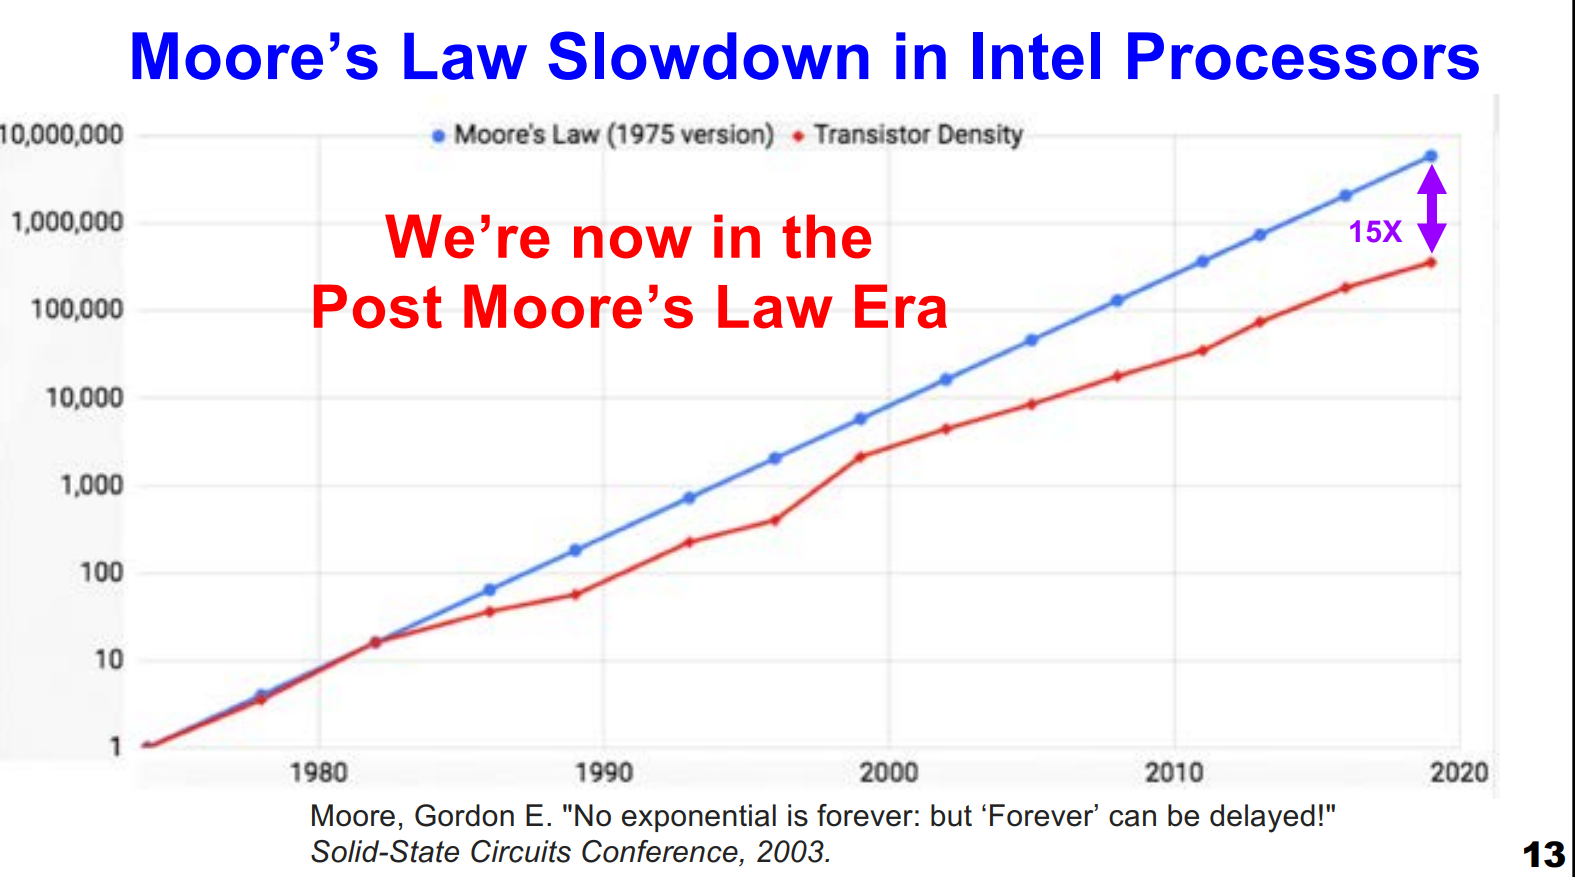
\includegraphics[width=0.85\textwidth]{images/mooreslaw.png}
    \caption{From "A Golden Age of Computers - David Patterson"
    \cite{patterson19}}
  \end{figure}

\end{frame}

\begin{frame}[fragile]
\frametitle{Problems Facing Modern Compute}
  \framesubtitle{Dennard Scaling}

  \begin{figure}
    \centering
    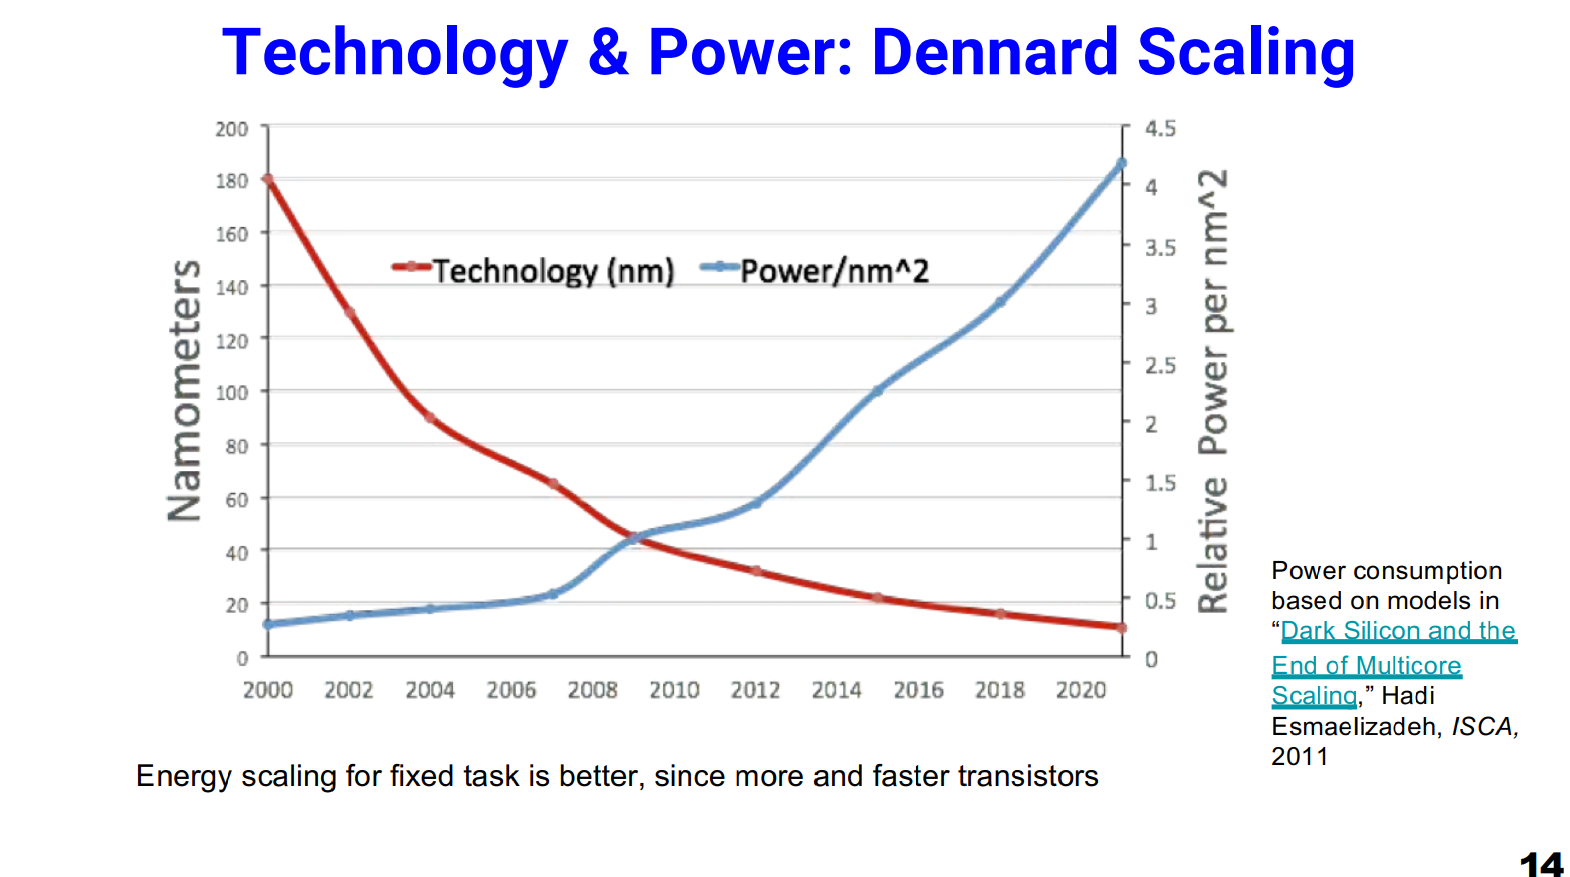
\includegraphics[width=0.85\textwidth]{images/dennardscaling.png}
    \caption{From "A Golden Age of Computers - David Patterson"}
  \end{figure}
\end{frame}

\begin{frame}[fragile]
\frametitle{Problems Facing Modern Compute}
  \framesubtitle{Von Neumann Bottleneck}

  \begin{figure}
    \centering
    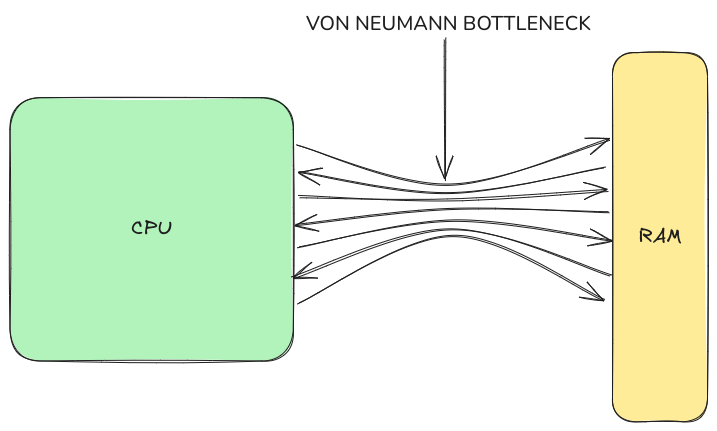
\includegraphics[width=0.85\textwidth]{images/vonneumann.png}
  \end{figure}
\end{frame}

\begin{frame}[fragile]
\frametitle{Overview of Modern Compute}
\framesubtitle{}
  \begin{itemize}
    \item ASICs are expensive to engineer, CPUs are slow, GPUs
      are power hungry and inflexible
    \item Should modern compute be restricted to CPUs/GPUs and a handful
      of ASICs?
    \item Following are four instances where existing compute falls short:
  \end{itemize}
\end{frame}

\begin{frame}[fragile]
\frametitle{Hard-to-Solve Problems for Modern Compute}
\framesubtitle{}
  \begin{itemize}
    \item Problems involving many peripherals and real-time compute
    \item Unusual Representation of Numbers (In contrast to fixed width) 
      (quantization for neural networks)
    \item New architectures/solutions for old problems (KANs)
    \item Power effiecient and flexible
  \end{itemize}
\end{frame}

\begin{frame}[fragile]
\frametitle{Problems Facing Modern Compute}
  \framesubtitle{}
  \begin{enumerate}
    \item The free lunch afforded by hardware improvements over years
      is coming to an end.
    \item New, creative, first-principles architectures and
      compute infrastrucutre need to be designed along with the
      software abstractions to use them. 
  \end{enumerate}
\end{frame}

\begin{frame}[c,fragile]
  \frametitle{}

  \centering
  \textbf{Chapter 2}
  \centering
  Introduction To Reconfigurable And Heterogeneous Computing
\end{frame}

\begin{frame}[fragile]
  \frametitle{Setting the stage}
  \framesubtitle{}
    Two key ideas:
      \begin{enumerate}
        \item Reconfiguration: The process through which a "reconfigurable
      processor" is re-programmed to implement a new circuit. Reconfiguration
          can be achieved by using circuits such as FPGAs.
    \item Heterogeneity: The idea that a system must include processors (such as
      CPUs/GPUs/DSPs/Other ASICs) of different 
          capacities/abilities well integrated together. Heterogeneity promotes
    \textcolor{green}{complementing} existing compute instead of
          \textcolor{red}{replacing}.
      \end{enumerate}
\end{frame}

\begin{frame}[fragile]
\frametitle{Key Problems With Reconfigurable-Heterogenous Computing}
\framesubtitle{}
    To implement a reconfigurable heterogeneous computer with FPGAs,
      the problems are two-fold:
  \begin{enumerate}
    \item Problem 1: Using FPGAs with traditional software is in-convenient.
    \item Problem 2: Writing new hardwares for FPGAs, implementing custom solutions is
      tedious with a very steep learning curve, often times requiring 
      domain expertise.
  \end{enumerate}
\end{frame}

\begin{frame}[fragile]
\frametitle{Reconfigurability: An Introduction to FPGAs}
\framesubtitle{}
  \begin{enumerate}
    \item Digital circuits are made up of gates and connections between
      them.
    \item FPGAs are a grid of programmable cells and switches that allows
      a user to create new gates and connections after the IC has been
      fabricated.
    \item Circuits for FPGAs are described using Hardware Descriptions Languages
      (HDLs) such as Verilog, VHDL.
    \item High level description of a circuit is compiled into real hardware
      (i.e. a representation that only uses FPGA primitives) by a "compiler".
  \end{enumerate}

\end{frame}


\begin{frame}[fragile]
\frametitle{Problem 1: Programming model for FPGAs}
\framesubtitle{}
  \begin{enumerate}
    \item A true programming model for FPGAs would heavily exploit
      reconfigurability.
    \item We introduce a non-Von Neumann flow-based reconfigurable architecture and a programming model
      for it.
  \end{enumerate}
\end{frame}

\begin{frame}[fragile]
  \frametitle{Comparison}
  \framesubtitle{}
  \begin{figure}
    \centering
    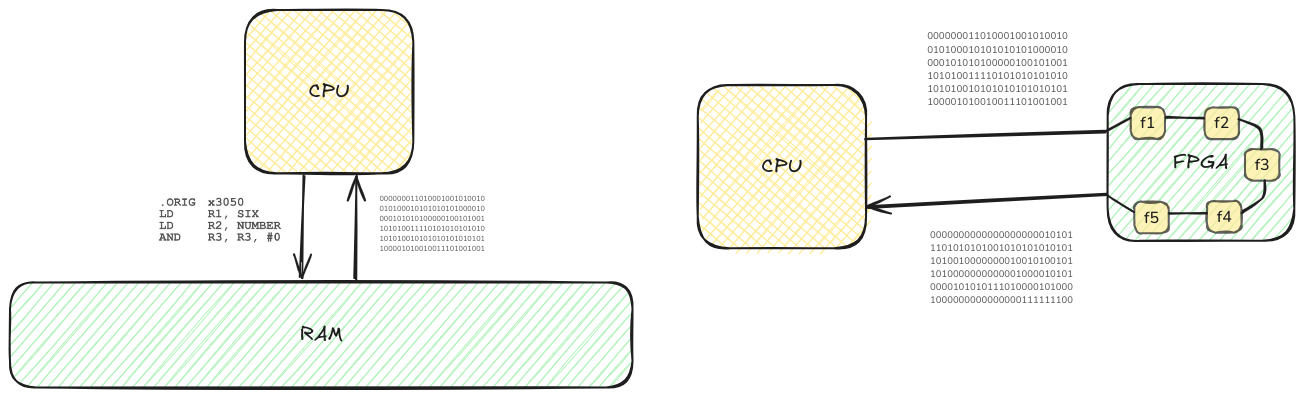
\includegraphics[width=1.0\textwidth]{images/flow.png}
    \caption{a) A Von-Neumann Computer b) A Flowing Reconfigurable Computer}
    \label{}
  \end{figure}
\end{frame}

\begin{frame}[fragile]
  \frametitle{Differences}
  \framesubtitle{}

  \begin{itemize}
    \item There are \textcolor{red}{no instructions} as the hardware
  is configured to a desired operation. 
      
    \item Data flows in and out of the chip transformed. 

    \item No instructions $\implies$ No ISA!

    \item "What to do with data" is a part of the hardware
  \end{itemize}
\end{frame}

\begin{frame}[fragile]
  \frametitle{An exemplary DSL for reconfigurable compute architectures}
\framesubtitle{}
  \begin{lstlisting}
    Base *input = new TensorSend("ts");
    Base *proc_one = new JPEGEncoderTillDct(input, "jpeg_encoder");
    Base *proc_two = new MlEngineCore(proc_one, "ml_core");
    Base *output = new TensorReceive(proc_two, "tr");
    Model m1 = new Model(input, output);
  \end{lstlisting}
\end{frame}

\begin{frame}[fragile]
  \frametitle{An exemplary DSL for reconfigurable compute architectures (2)}
\framesubtitle{}
  \begin{lstlisting}
    m1->compute(input);
    if (some_user_defined_condition(m1->output())) {
      m2->compute(m1->output());
    } else {
      return m1->out();
    }
  \end{lstlisting}
  \texttt{model->compute} is the function that triggers generation, flashing and
  computation on a hardware described by a Model.

  The code above demonstrates \textit{conditional reconfiguration}.
\end{frame}

\begin{frame}[fragile]
  \frametitle{An exemplary DSL for reconfigurable compute architectures (3)}
\framesubtitle{Continue}
   \begin{figure}
        \centering
        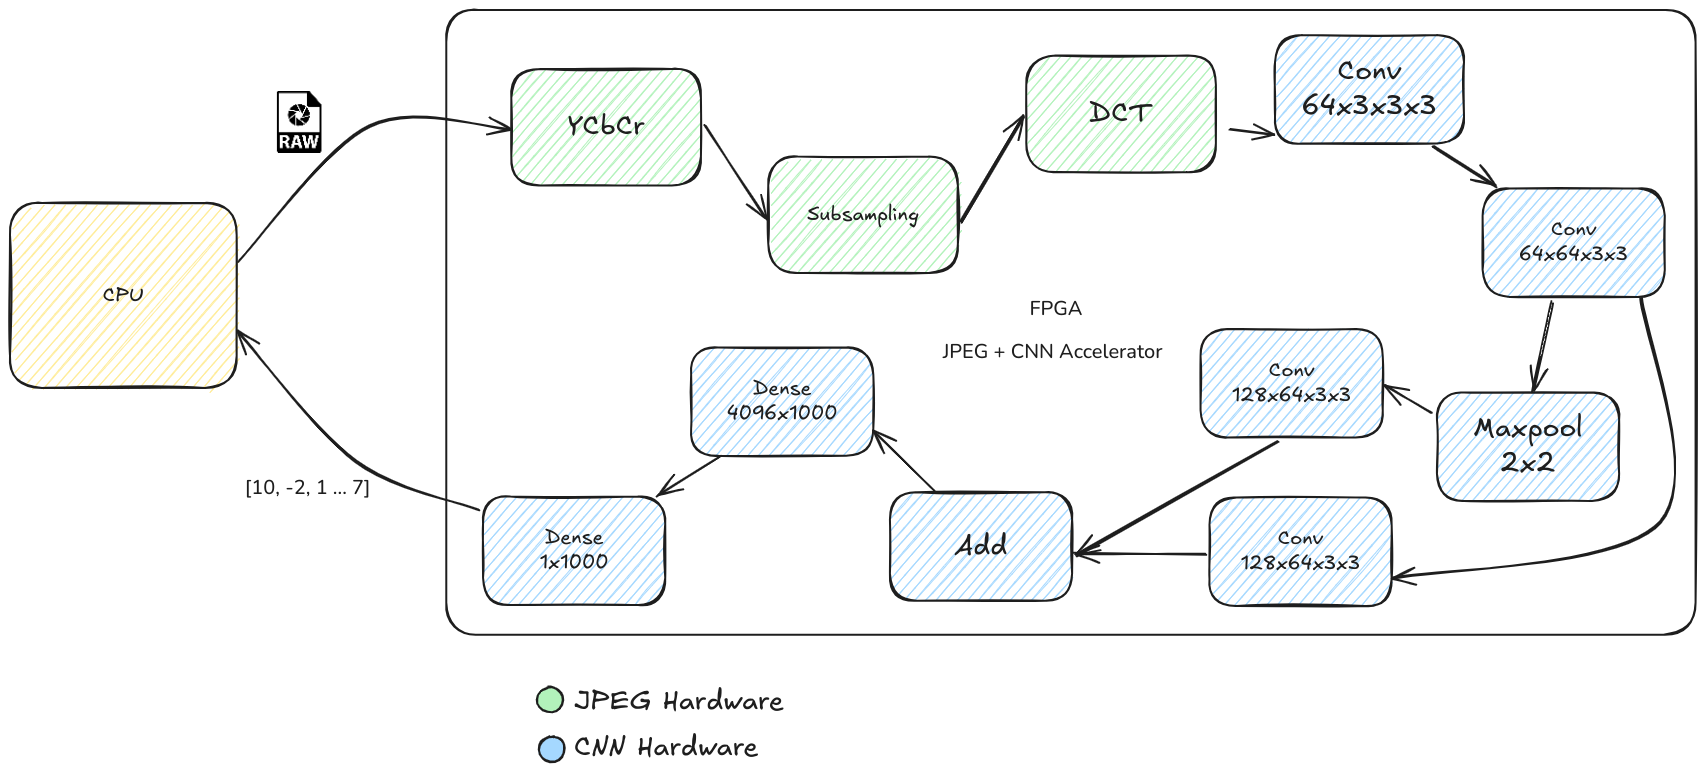
\includegraphics[width=1\linewidth]{images/flowcnnjpeg.png}
        \caption{Data flow for JPEG (Partial) + CNN inference}
    \end{figure}
\end{frame}


\begin{frame}[c,fragile]
  \frametitle{}

  \centering
  \textbf{Chapter 3} 
  \centering
  Need for modern EDA Compilers
\end{frame}

\newcommand\myheading[1]{%
  \par\bigskip
  {\Large\bfseries#1}\par\smallskip}

 
\begin{frame}[fragile]
  \frametitle{Problem 2: Writing Hardware Is Hard}
  \framesubtitle{}
  \begin{enumerate}
    \item Hardwares are written using HDLs like Verilog/VHDL
    \item Problems can be categorized as those above HDL level and those below
    \item Problems above HDL are solved by new tools and frameworks that
      such HDL wrappers (SpinalHDL, Chisel etc), High-Level Synthesis tools
      (name them), simulators/verifiers (verilator, CIRCT etc.)
    \item We are particularly interested in solving problems below HDLs.

    \item EDA tools are propreitary and hard-to-work-with.
    \item The general problem of compilation of hardwares is NP-Complete but
      there are special cases that can be exploited.
  \end{enumerate}
\end{frame}

\begin{frame}[fragile]
  \frametitle{FPGA CAD Toolflow}
  \framesubtitle{}
   \begin{figure}
        \centering
        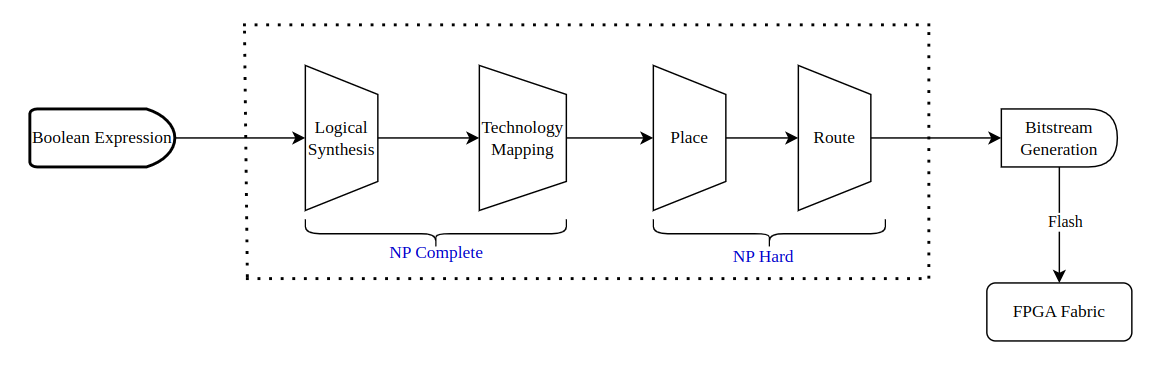
\includegraphics[width=1\linewidth]{images/cad_flow.png}
        \caption{FPGA CAD Tool Flow}
        \label{exa_cadflow}
    \end{figure}
\end{frame}

\begin{frame}[fragile]
  \frametitle{FPGA CAD Toolflow}
  \framesubtitle{}
   \begin{itemize}
     \item Logical Synthesis: HDL to primitive gates (AND/OR).
     \item Technology Mapping: Mapping generic AND/OR gates to k-LUTs.
     \item Placement: Placing k-LUTs in a constrained grid representing the FPGA
       based on a cost model
     \item Routing: Connection placed LUTs so that the latency is minimum
     \item Bitstream Generation: Generating a final bitstream that the FPGA
       can understand.
    \end{itemize}
\end{frame}

\begin{frame}[fragile]
  \frametitle{The Current State of EDA tools}
  \framesubtitle{}
  \begin{enumerate}
    \item Like the FPGA architectures, tools to work with them are propreitary.
    \item Problems and sub-problems in the flow are ridden with NP-Hard and
      NP-Complete problems.
    \item There is a gap between CAD research and production ready CAD tools.
  \end{enumerate}
\end{frame}

\begin{frame}[fragile]
  \frametitle{Optimization Opportunities for EDA Compilers}
  \framesubtitle{}
  \begin{enumerate}
    \item Our DSL compiler connects hardware together. The mapping phase
      of hardware generation can be completely bypassed if The compiler can
      be designed to operate on netlists directly instead of verilog.
    \item The mapping process involves, among many steps, a phase where it looks
      for a minimal boolean expression. In iterative write-compile-debug loops
      entire hardware may not change frequently so their resulting minimal
      boolean expressions history can be saved and revisited for next
      iterations.
    \item Routing can be designed to make use of GPUs.
  \end{enumerate}
\end{frame}

\begin{frame}[c,fragile]

  \centering
  \textbf{Chapter 4}
  Work Done Towards Implementation
\end{frame}

\begin{frame}[fragile]
  \frametitle{Realizing this goal}
  \begin{enumerate}
    \item Realizing this goal requires design and implementation from
      first principles.
    \item To achieve this, we designed our own hardware: Vaaman. 
    \item Vaaman is a reconfigurable heterogenous computer.
  \end{enumerate}
  \framesubtitle{}
\end{frame}

\begin{frame}[fragile]
  \frametitle{The Hardware (Vaaman)}
  \framesubtitle{}
  \begin{figure}
    \centering
    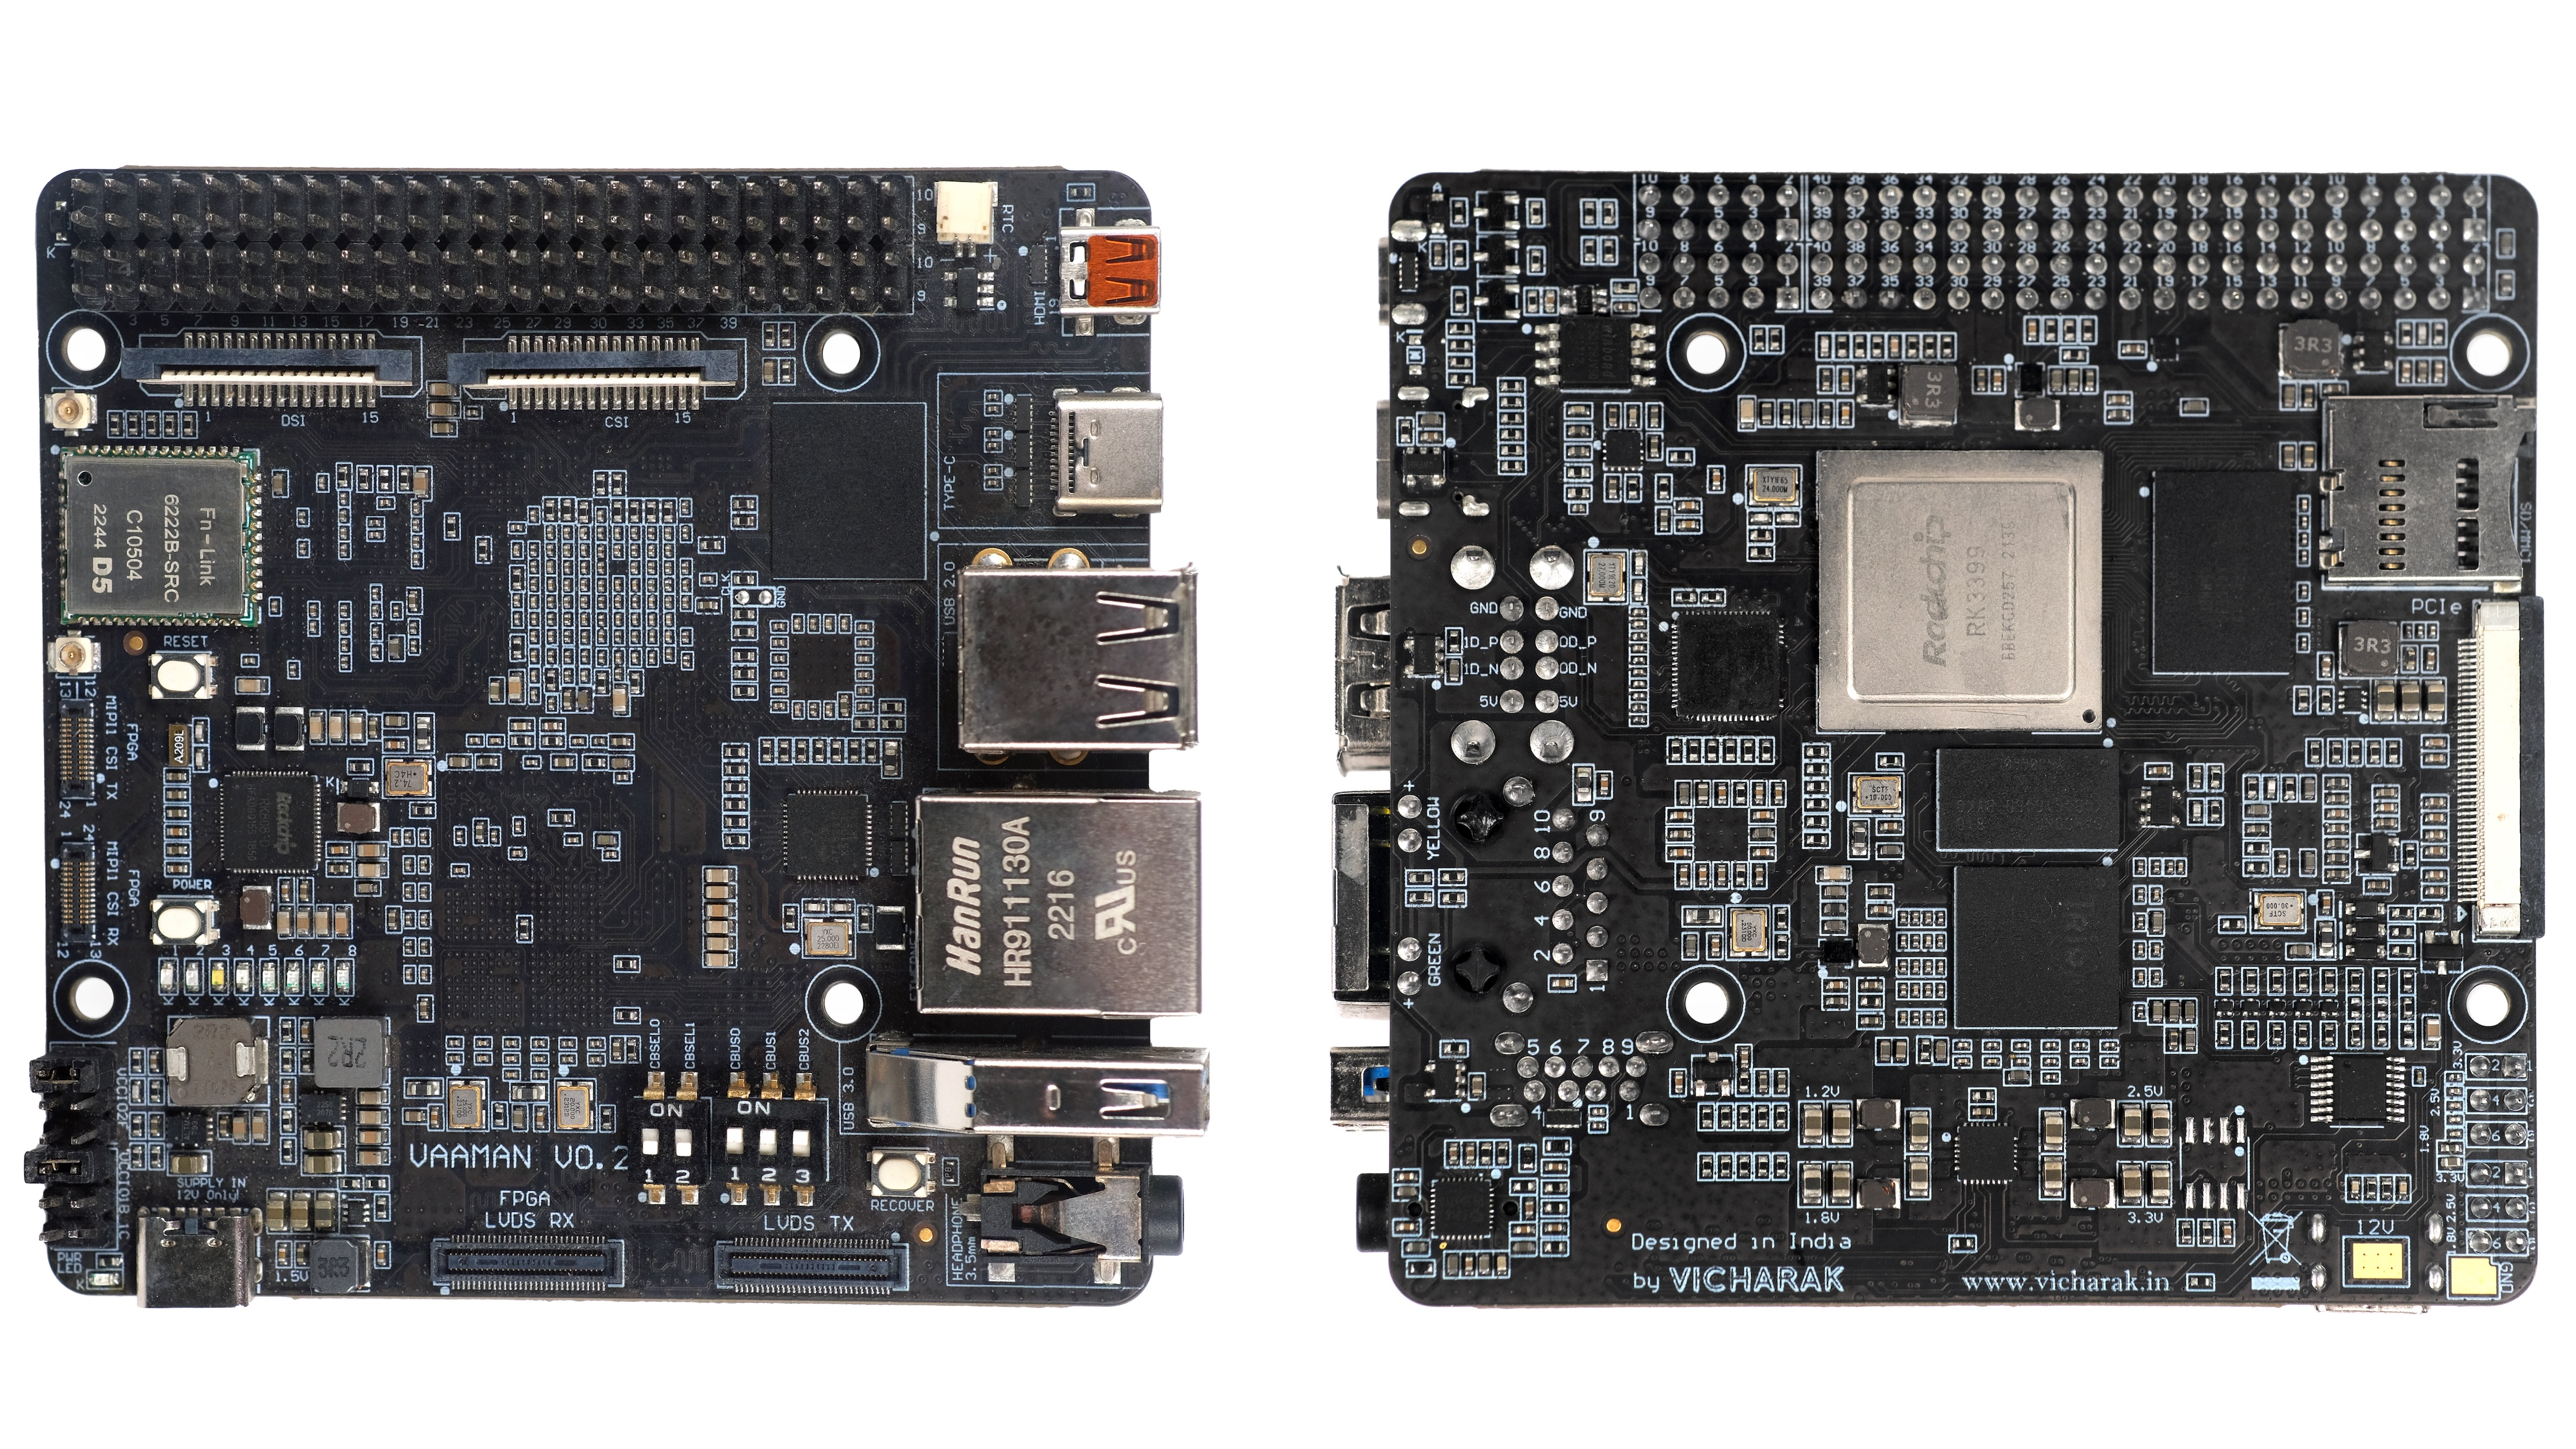
\includegraphics[width=0.95\textwidth]{vaaman.jpg}
    \caption{Vaaman: A heterogenous SBC \\ \url{https://shorturl.at/5y9QA}}
    \label{neuron}
  \end{figure}
  
\end{frame}

\begin{frame}[fragile]
  \frametitle{ML Accelerator (Gati)}
  \begin{itemize}
    \item Gati is a set of hardware and software programs that perform CNN
  acceleration with FPGA as a co-processor on Vaaman.
\item Gati accelerates MAC operations with a Systolic-Array based MAC engine,
  and handles control flow with a macro-ISA.
    \item Compiler parses protobufs, performs transpositions, and generates
      instructions for execution. It can also generate custom hardware for
      each model.
    \item The runtime partitions a network into execute-on-host and
      execute-on-device, re-orders inputs, and offloads computation
      to the FPGA.
  \end{itemize}
\end{frame}

\begin{frame}[fragile]
  \frametitle{Periplex - On-the-Fly Peripheral Generation}
  \begin{itemize}
    \item Hardware peripherals are limited by fabrication at the ASIC level or
      in MCUs and MPUs.
    \item Emerging embedded industries like drones, autonomous
  vehicles, industrial gateways, robotics require more hardware peripheral
  accessibility and innovation due to real-time operations.
    \item Periplex allows software-defined generation of peripherals on
      reconfigurable hardware (FPGAs) with JSON-driven configuration and
      integrated drivers directly in the linux kernel so they can be
      accessed easily.
  \end{itemize}
\end{frame}

\begin{frame}[fragile]
  \frametitle{Conclusion}
  \framesubtitle{}

  \begin{enumerate}
    \item Reconfigurable architectures can provide a way to solve many problems
      that existing compute struggle with and help alleviate the von-neumann
      bottleneck.
    \item Heterogenous approach of assisting instead of replacing integration of
      new hardwares in systems can allow existing infrastructure to be used.
    \item Two of the biggest problems with achieving this are a) programming
      model that exploits reconfigurability b) fast and flexible hardware
      compilers (EDA tools).
    \item Solutions to problem a) manifest themselves in the form of novel DSLs
      and compiler/runtime toolchains compatible with current
      toolchain/workflows used by CPUs.
    \item Solutions to problem b) involve finding optimization oppurtunities
      to speed up EDA tools, making use of modern parallel hardwares such as
      GPU, and other accelerators.
  \end{enumerate}
\end{frame}

\begin{frame}[fragile]
  \frametitle{}
  \framesubtitle{}

  Extended slides and more stuff: 

  \begin{verbatim}
  github.com/vicharak-in/noisa
  \end{verbatim}

  We are hiring! Email us at: 

  \begin{verbatim}
  join-the-team@vicharak.in
  \end{verbatim}

\end{frame}

}

\end{document}
